\documentclass{standalone}
\usepackage{graphicx}	
\usepackage{amssymb, amsmath}
\usepackage{color}

\usepackage{tikz}
\usetikzlibrary{intersections, backgrounds}

\definecolor{light}{RGB}{220, 188, 188}
\definecolor{mid}{RGB}{185, 124, 124}
\definecolor{dark}{RGB}{143, 39, 39}
\definecolor{highlight}{RGB}{180, 31, 180}
\definecolor{gray10}{gray}{0.1}
\definecolor{gray20}{gray}{0.2}
\definecolor{gray30}{gray}{0.3}
\definecolor{gray40}{gray}{0.4}
\definecolor{gray60}{gray}{0.6}
\definecolor{gray70}{gray}{0.7}
\definecolor{gray80}{gray}{0.8}
\definecolor{gray90}{gray}{0.9}
\definecolor{gray95}{gray}{0.95}

\newcommand*{\offset}{0.025}

\begin{document}

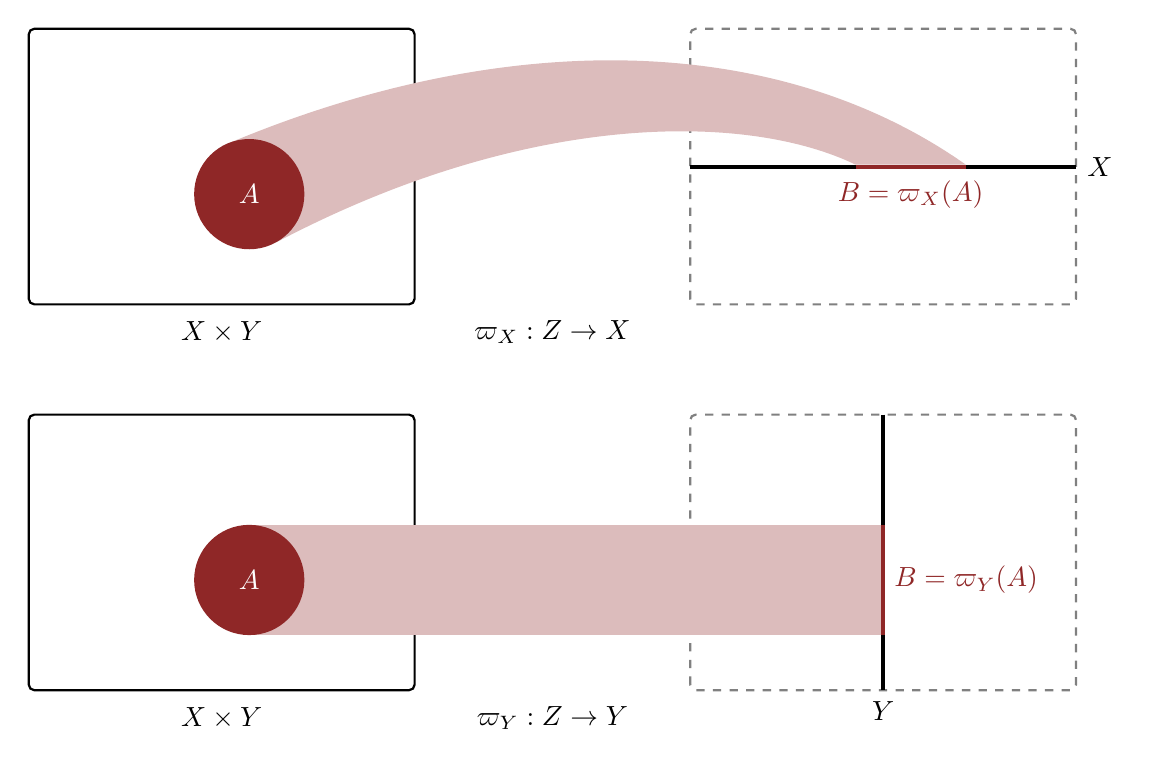
\begin{tikzpicture}[scale=0.35, thick]

  \draw [rounded corners=2pt, color=black] (-5, 0) rectangle +(-14, 10);
  \node at (-12, -1) { $X \times Y$ };

  \draw [rounded corners=2pt, color=gray, dashed] (5, 0) rectangle +(14, 10);
  
  \node at (0, -1) { $\varpi_{X}: Z \rightarrow X$ };
  
  \draw [line width=1.5] (5, 5) -- +(14, 0)
  node[right] { $X$ };
  
  \fill [color=light] (-10, 2.26) -- (-12, 5.74) .. controls (-2, 10) and (8, 10) .. 
                      (15, 5.07) -- (11, 5.07) .. controls (7, 7) and (-1, 7) .. (-10, 2.26);
  
  \fill [fill=dark, text=white] (-11, 4) circle (2)
  node { $A$ };
 
  \draw [color=dark, text=dark, line width=1.5] (11, 5) -- (15, 5)
  node[midway, yshift=-10] { $B = \varpi_{X}(A)$ };
  
  %
  \draw [rounded corners=2pt, color=black] (-5, -14) rectangle +(-14, 10);
  \node at (-12, -15) { $X \times Y$ };

  \draw [rounded corners=2pt, color=gray, dashed] (5, -14) rectangle +(14, 10);
  
  \node at (0, -15) { $\varpi_{Y}: Z \rightarrow Y$ };
  
  \draw [line width=1.5] (12, -4) -- +(0, -10)
  node[below] { $Y$ };
  
  \fill [color=light] (-11, -12) -- (-11, -8) -- (12, -8) -- (12, -12) -- cycle;
  
  \fill [fill=dark, text=white] (-11, -10) circle (2)
  node { $A$ };
  
  \draw [color=dark, text=dark, line width=1.5] (12, -8) -- (12, -12)
  node[midway, xshift=30] { $B = \varpi_{Y}(A)$ };
  
    
\end{tikzpicture}

\end{document}  